% Can Language Models Learn Forever? Stationarity and Plasticity Under Continual Pretraining
% An endless data stream feeds one language model, which must balance plasticity and stationarity.
\documentclass[tikz,border=0pt]{standalone}
% Shared look for the TikZ publication thumbnails.
% Canvas: 16cm x 10cm (16:10, matching the 640x400 WebP output), white, site palette.
% Labels are large (\lbl) because thumbnails are shown about 200px wide.
\usepackage[T1]{fontenc}
\usepackage{helvet}
\renewcommand{\familydefault}{\sfdefault}
\usepackage{amsmath,amssymb}
\usepackage{fontawesome5}
\usetikzlibrary{arrows.meta,calc,positioning,shapes.geometric,shapes.callouts,decorations.pathmorphing,shadows}

\definecolor{ink}{HTML}{2B2D42}
\definecolor{accent}{HTML}{B509AC}
\definecolor{teal}{HTML}{1E9BC0}
\definecolor{violet}{HTML}{6C5CE7}
\definecolor{orange}{HTML}{F28C28}
\definecolor{sun}{HTML}{F2C14E}
\definecolor{leaf}{HTML}{2CA58D}
\definecolor{alert}{HTML}{E5484D}
\definecolor{mist}{HTML}{EEF0F5}

\tikzset{
  every picture/.append style={line cap=round, line join=round},
  card/.style={rounded corners=10pt, draw=#1!75!black, line width=1.4pt, fill=#1!12},
  arrow/.style={-{Stealth[length=10pt,width=9pt]}, line width=2.2pt, draw=#1},
  soft shadow/.style={drop shadow={shadow xshift=0pt, shadow yshift=-3pt, opacity=0.18, fill=ink}},
  badge/.style={circle, fill=#1!14, draw=#1, line width=2pt, minimum size=2.3cm, text=#1},
}
\newcommand{\thumbcanvas}{\useasboundingbox[fill=white] (0,0) rectangle (16,10);}
\newcommand{\lbl}[1]{{\fontsize{20}{22}\selectfont\bfseries #1}}
\newcommand{\icon}[2][34]{{\fontsize{#1}{#1}\selectfont\faIcon{#2}}}
% Window chrome: dark editor panel with traffic-light dots. Args: x0, y0, x1, y1.
\newcommand{\editor}[4]{%
  \fill[ink, rounded corners=12pt, soft shadow] (#1,#2) rectangle (#3,#4);
  \foreach \c [count=\k] in {alert,sun,leaf} \fill[\c] ({#1+0.15+0.42*\k},{#4-0.42}) circle (0.13);
}

\begin{document}
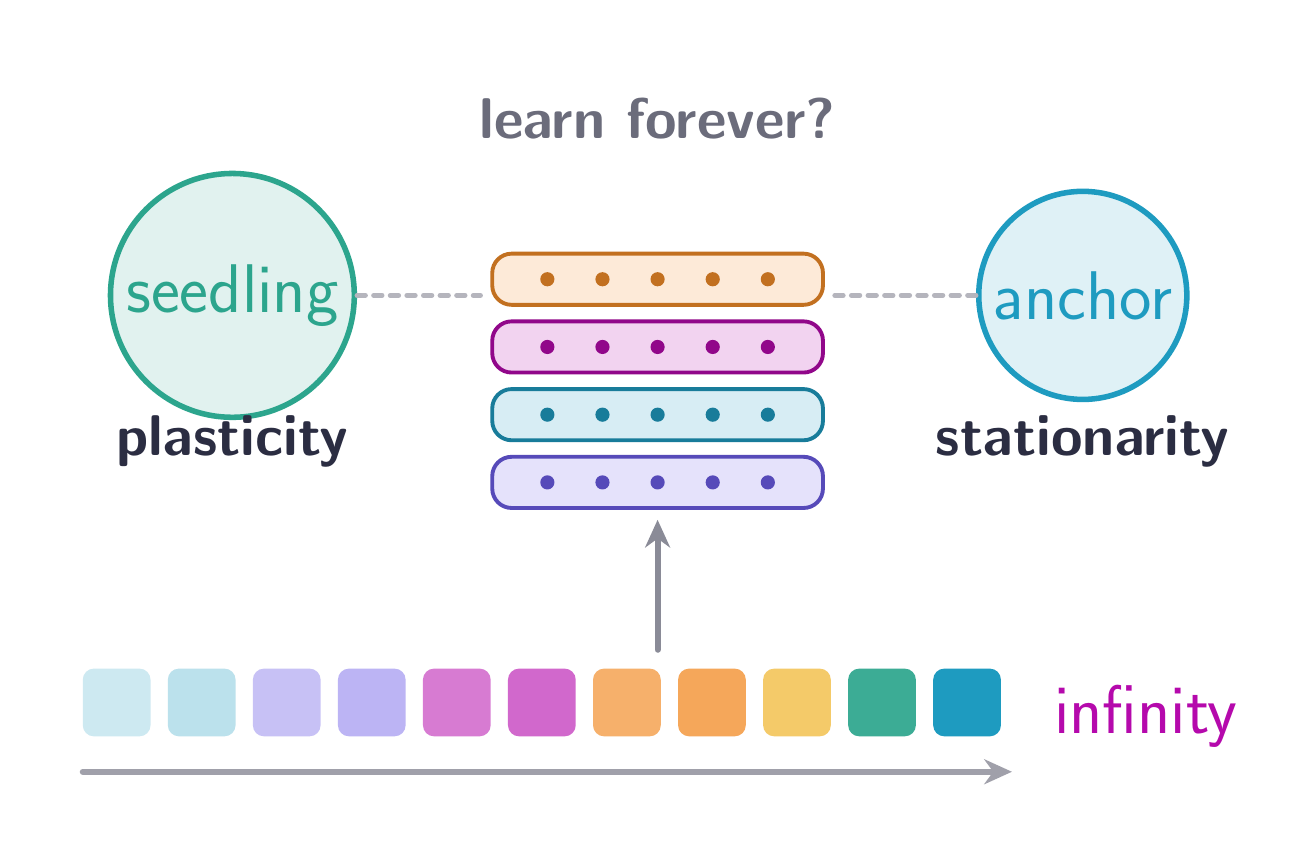
\begin{tikzpicture}
\thumbcanvas
% Data stream: older shards fade, the stream never ends.
\foreach \c [count=\i from 0] in {teal,teal,violet,violet,accent,accent,orange,orange,sun,leaf,teal} {
  \pgfmathsetmacro{\op}{0.22+0.078*\i}
  \fill[\c, opacity=\op, rounded corners=4pt] ({0.7+\i*1.08},1.0) rectangle ++(0.86,0.86);
}
\draw[arrow=ink!45] (0.7,0.55) -- (12.5,0.55);
\node[text=accent] at (14.2,1.25) {\icon[46]{infinity}};
% The language model: a stack of layers.
\foreach \c [count=\k from 0] in {violet,teal,accent,orange} {
  \draw[line width=1.4pt, draw=\c!80!black, fill=\c!18, rounded corners=7pt]
    (5.9,{3.9+\k*0.86}) rectangle (10.1,{4.55+\k*0.86});
  \foreach \n in {0,...,4} \fill[\c!80!black] ({6.6+\n*0.7},{4.225+\k*0.86}) circle (0.09);
}
\draw[arrow=ink!55] (8,2.1) -- (8,3.75);
% The two competing goals.
\node[badge=leaf] (P) at (2.6,6.6) {\icon{seedling}};
\node[text=ink] at (2.6,4.75) {\lbl{plasticity}};
\node[badge=teal] (S) at (13.4,6.6) {\icon{anchor}};
\node[text=ink] at (13.4,4.75) {\lbl{stationarity}};
\draw[line width=1.8pt, dashed, ink!35] (P.east) -- (5.75,6.6);
\draw[line width=1.8pt, dashed, ink!35] (S.west) -- (10.25,6.6);
\node[text=ink!70] at (8,8.85) {\lbl{learn forever?}};
\end{tikzpicture}
\end{document}
